
\section{Challenges to the Liberal Order: Summary}
\begin{center}
\textit{David A. Lake, Lisa L. Martin, and Thomas Risse (2021)}
\end{center}

\subsection{Introduction and Central Argument}

The Liberal International Order (LIO) is under pressure from several directions at once. The authors emphasize that the postwar order has survived serious crises before, so its collapse should not be assumed.

The LIO has structured relations among the capitalist, democratic, and industrialized states since the late 1940s and has had wider global effects. It is associated with unprecedented cooperation among North America, Western Europe, and Japan, the emergence of a pluralistic security community, expansion of trade and capital mobility, high economic growth, the diffusion of democracy, and the development of an international human-rights regime.

\subsection{Order}

An order consists of patterned or structured relations. The LIO is clearly rule-governed and sustained by coordinated action by both state and nonstate actors.

\subsection{International and the Westphalian Order}

The "international" component of the LIO has to be understood in relation to the Westphalian order. In the authors' usage, Westphalia is not literally a system created in 1648 but a later order centered on sovereign nation-states, sovereign equality, recognition by other states, and noninterference in domestic affairs. The LIO and the Westphalian order partly overlap and have coevolved since 1945. They share principles such as sovereign equality, peaceful settlement of disputes, self-determination, and nonintervention. At the same time, the LIO goes beyond Westphalia through principles such as human rights and forms of legitimate collective intrusion into domestic affairs.

\begin{center}
    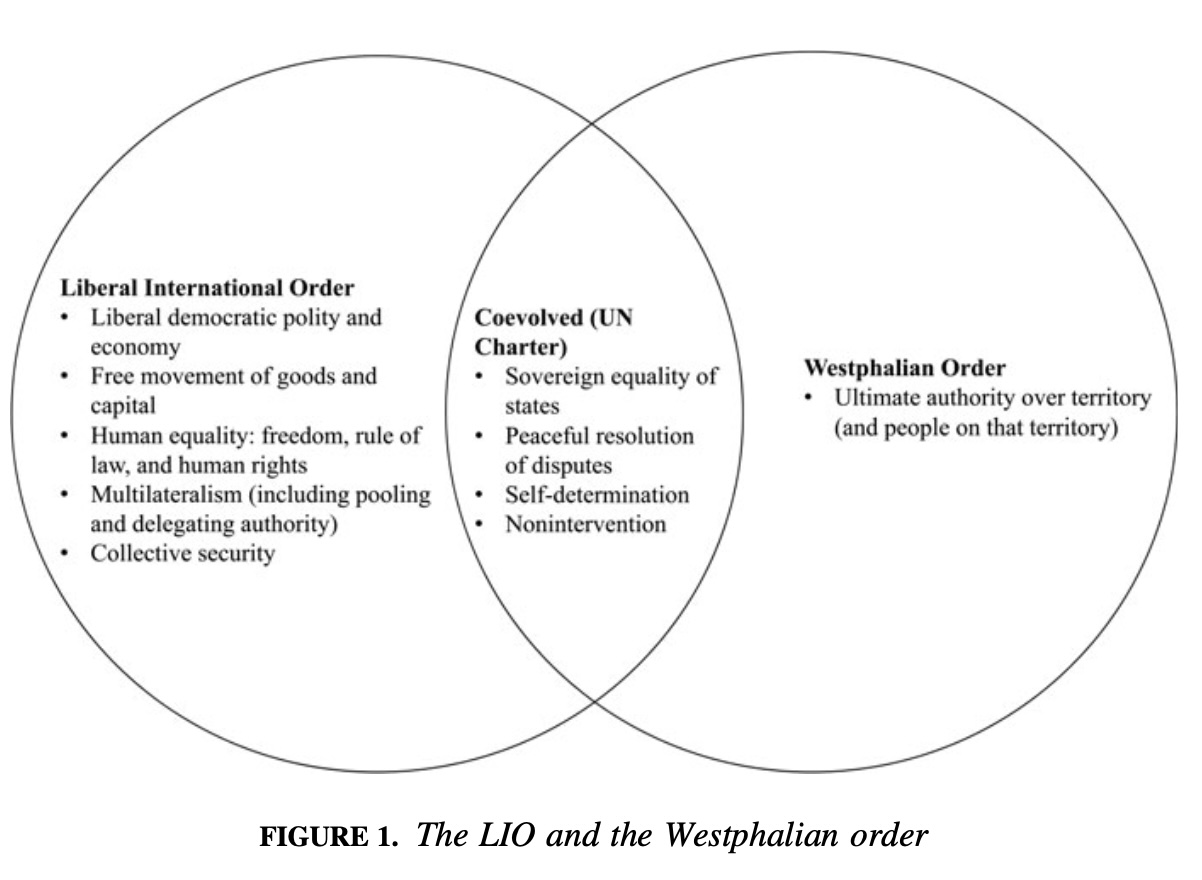
\includegraphics[width=1\textwidth]{images/challenges_to_liberal_order_LIO_vs_westphalian.jpg}
    \captionof{figure}{\label{fig:fig6_challenges_to_liberal_order_LIO_vs_westphalian.jpg}%\textit{\parencite[Fig.\(\backsim\)1]{cranmerWhatCanWe2017}}
    }
\end{center}

\subsection{Liberal: Political Liberalism}
At its philosophical core, liberalism rests on universal human equality, freedom, and individual and collective self-determination. Political liberalism therefore implies the rule of law, representative government, political participation, and protection of individual rights.

Institutions such as the International Criminal Court and doctrines such as the Responsibility to Protect illustrate how the LIO can authorize constraints on domestic sovereignty in the name of universal rights.

\subsection{Economic Liberalism and Embedded Liberalism}

A classical version favors market capitalism, free trade, international capital mobility, and equal treatment of foreign investment.

A second, historically important version is embedded liberalism. The postwar architects of the Bretton Woods system combined trade liberalization with domestic welfare states.

The distinction is important because economic liberalism does not automatically contradict Westphalian sovereignty.

The LIO broadly liberalized goods, services, and capital but never generally established free movement of labor outside the EU.

\subsection{Liberal Internationalism}

The institutional dimension of the LIO is based on principled multilateralism. Multilateralism means more than coordination among several states: it means coordination according to generalized rules that apply across cases rather than ad hoc bargaining based solely on particular interests. The GATT,WTO and UN Charter exemplify this logic. Liberal internationalism also includes peaceful dispute resolution, the ambition to provide global public goods, security communities such as NATO, and multilateral arms-control and nonproliferation regimes.

\textbf{Tensions with Westphalia:}
\begin{enumerate}
    \item Authority is delegated supranational bodies
    \item Majority voting
    \item Dispute-settlement mechanisms
    \item International courts.
\end{enumerate}

\subsection{Universalism and Selective Participation}

The LIO contains a paradox. Because liberalism begins from universal equality, the order is in principle open to all states. Yet states can join important parts of the LIO without being liberal democracies.

The LIO is therefore best understood as an evolving order whose components vary in reach rather than as a single uniform system imposed everywhere by the United States.

\subsection{Challenges from Within the Liberal Core}

The most striking contemporary threats come not only from geopolitical rivals but also from the internal workings of liberalism itself. The authors identify several mechanisms through which the LIO generates opposition within its own core members.

\begin{enumerate}
    \item Economic liberalism creates winners and losers. Trade openness, technological change, global production chains, and the financial crisis of 2008--2010 have produced geographically concentrated losses and contributed to rising inequality.
    \item Political openness can be used against liberalism. Freedom of expression and the open architecture of the internet allow misinformation, foreign influence, and strategies of "truth subversion" to circulate widely. 
    \item Free-trade policies and supranational governance were sometimes insulated from popular pressure in order to prevent protectionism and secure long-term cooperation. Over time, however, this technocratic insulation excluded some constituencies and created resentment. International institutions appeared less responsive to citizens.
    \item liberal universalism collides with national identity. Who belongs to the national community? Migration is a problem
\end{enumerate}

\subsection{Nationalist Populism and Political Realignment}

These pressures converge in movements combining nationalism, populism, and authoritarianism. Nationalism prioritizes the interests and identity of a particular state; populism pits a supposedly homogeneous "people" against elites and pluralist institutions; authoritarianism rejects liberal constraints such as independent courts, a free press, and fair electoral competition.

\subsection{External Challengers}

\begin{itemize}
    \item Climate change
    \item Distributional conflicts due to Climate change
    \item China: Its extraordinary economic growth was enabled by participation in the open international economy, yet China remains authoritarian and strongly defends sovereignty and noninterference.
\end{itemize}

\subsection{The Erosion of Multilateral Institutions}

Internal and external challenges converge most directly in attacks on multilateralism. Multilateral institutions have experienced crises before, including the collapse of the Bretton Woods monetary system and the US decision to invade Iraq without broad UN support. What appears different in the contemporary period is the breadth of skepticism and the willingness of major states to weaken institutions without a clear systemic necessity.

\begin{enumerate}
    \item WTO crisis: Even before the recent crisis it struggled to negotiate large new trade agreements. The United States combined protectionist tariffs with a strategy of blocking appointments to the WTO Appellate Body, impairing enforcement.
    \item Refugee crisis: The refugee regime illustrates a broader erosion of multilateral commitments. The principle of nonrefoulement and the 1951 Refugee Convention created legal obligations toward asylum seekers, yet receiving states have increasingly adopted restrictive or deterrent policies.
\end{enumerate}

\subsection{Sources of Resilience}

\begin{enumerate}
    \item the order has produced substantial benefits: reduced conflict among core members, economic growth, lower global poverty, and extensive international cooperation.
    \item LIO has generated vested interests: Firms have built global investments and supply chains that depend on open trade and predictable international rules. The same interdependence that creates vulnerability can also reinforce support for openness.
    \item the LIO institutions can outlast the circumstances that produced them and act as shock absorbers during crises.
    \item \textbf{Legitimacy}: After decades of operation, many rules of multilateral cooperation have acquired a sense of normality and rightfulness. Practices that once required active justification can become taken for granted as normal components of international life.
    
    \textbf{Accumulated normative capital}
    
    \textbf{Political baseline}
\end{enumerate}

\subsection{Four Analytic Blind Spots in IR Scholarship}

\begin{enumerate}
    \item \textbf{Exclusion}, stigma, and the threat of losing membership help enforce order. Exclusion is not merely a defect at the margins of the LIO.
    \item \textbf{Orders Are Not Neutral:} distributional consequences and the fact that rules are written by particular actors for particular purposes. Cooperation can be Pareto-improving while still distributing gains unequally.
    \item \textbf{Institutions Depend on Social Foundations:} Institutions survive because social groups invest political resources in creating and defending them. Institutional insulation may sometimes be necessary to protect long-term cooperation from short-term pressures.
    \item \textbf{Domestic Politics Can Challenge the Order Itself:} IR scholarship  paid little attention to the possibility that parties, protest movements, territorial cleavages, and mass political realignments inside core states could attack the international order itself.
\end{enumerate}

\subsection{USA and the Future of LIO}
Question about American leadership.

\begin{itemize}
    \item The LIO could survive because existing institutions and old and new stakeholders defend it.
    \item more traditional Westphalian order centered on sovereignty and noninterference.
    \item It could be transformed into a hybrid order that preserves economic openness and principled multilateralism while altering commitments to democracy, human rights, and international legal authority.
\end{itemize}